
\subsection*{\textbf{Question 4.c)}}
\begin{quote}

\textbf{Problem}
\begin{quote} 
Use the Zeldovich approximation to generate a movie of the evolution of a volume in two dimensions
from a scale factor of 0.0025 until a scale factor of 1.0. To do this, start with 64x64 particles arranged in a square grid with a grid spacing of 1 Mpc. Use $P(k) = k^{-2}$ and the given equation to generate $c_k$, then use the FFT on your grid of particles to calculate $\textbf{S(q)}$. As $a$ increases, update the positions and momenta of the particles and save each step as a frame for your movie. 
\end{quote}

\textbf{Solution} 
\begin{quote}
The difficulty of this exercise lays by the calculation the components of the displacement vector. A brief description of how this is done can be found below.
\\

The displacement vector is calculated by first creating a matrix in $k$ -space with complex values based on the given power law (similar to exercise 2). The matrix is next given the correct hermitian symmetry (see again exercise 2). The components of the displacement vector, $s_x$ and $s_y$, are then calculated independent with the help of this matrix.  This calculation is done as follows. The hemitian matrix is copied and the components in the matrices are multiplied with the wavenumbers and the complex number $i$. The wavenumbers by which the components are multiplied depends on whether we want $s_x$ or $s_y$. The result is two matrices where the cells have respectively values of $ic_k k_x$ and $ic_k k_y$. After this multiplication the matrices cannot be directly fourier transformed to obtain $s_x$ and $s_y$, as the multiplication with the wavenumbers breaks the symmetry in the columns with nyquest wavenumbers. The symmetry is only broken by a minus sign and this is corrected before doing the IFFT. 
\\
The code that creates the movie and the plots for the first 10 particles can be found below. The final plot of the movie is also included and shows that the particles clearly move to the denser region (see figure 25 on page 47).

\end{quote}
\newpage


\textbf{Code - Plots}:
\begin{quote}

The code that creates the movie and the plots of the first 10 particles. The code does make use of an object called 'random' and a function called \texttt{gen\_ complex}. This object and the function  can be found on page 53. The code for the imported shared modules can also be found at page 53. The movie can be found in the movie folder.
\lstinputlisting[firstline = 98, lastline=227]{./Code/assigment_4.py}
\end{quote}

\newpage

\textbf{Plots - Field}

\begin{quote}
\begin{figure}[!ht]
\centering
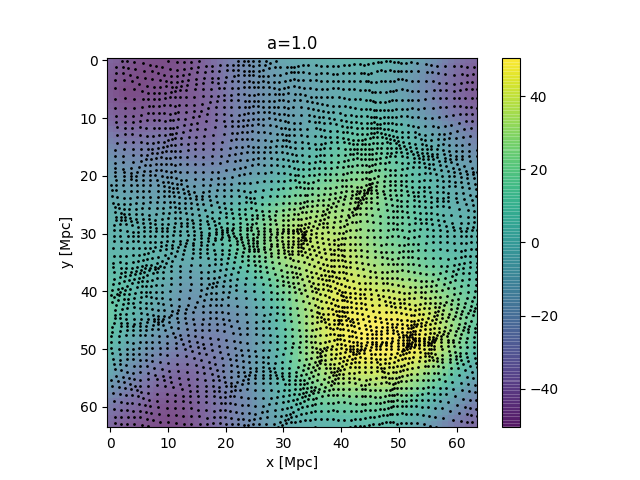
\includegraphics[width=14cm, height=9.5cm]{./Plots/4c/4c=89.png}
\caption{The final plot of the movie. It can clearly be seen that the particles (black dots) moved to the denser region. }
\label{FIG:stuff}
\end{figure}
\end{quote}

\textbf{Plots - particles}
\begin{quote}
\begin{figure}[!ht]
\centering
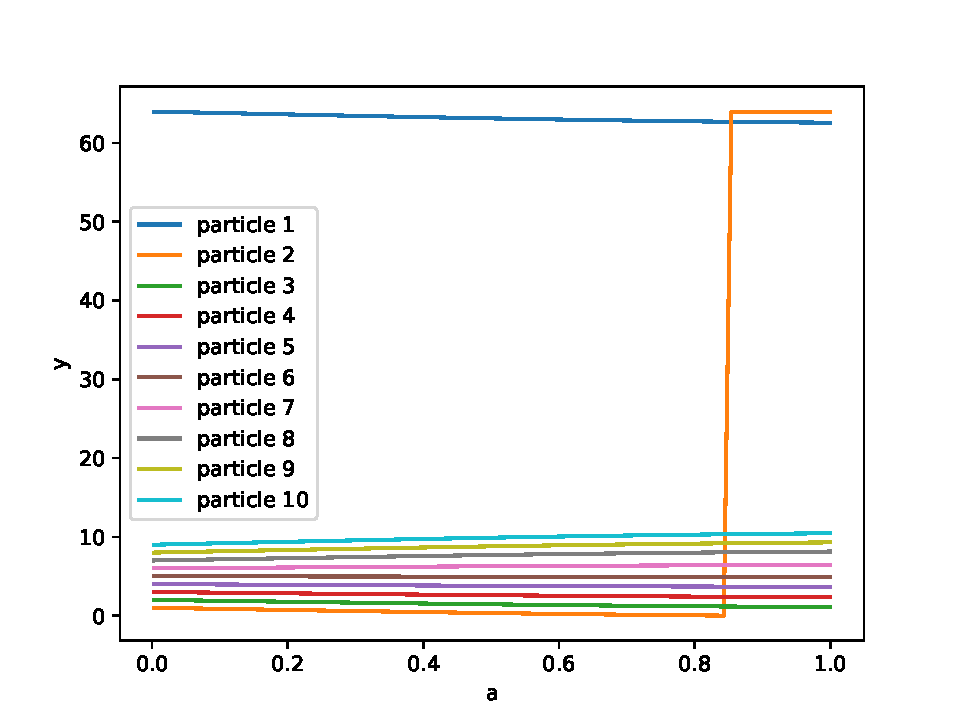
\includegraphics[width=14cm, height=8.5cm]{./Plots/4c_pos.pdf}
\caption{The y-positions of the first 10 particles as function of the scale factor. The plot shows that the particles are slowly moving to a denser region (see figure 25, where the first 10 particles are at the left top). The large jump for particle 2 (orange) at a scale factor of around $ a \approx 0.8$ is the result of the circular boundary conditions.  }
\end{figure}

\begin{figure}[!ht]
\centering
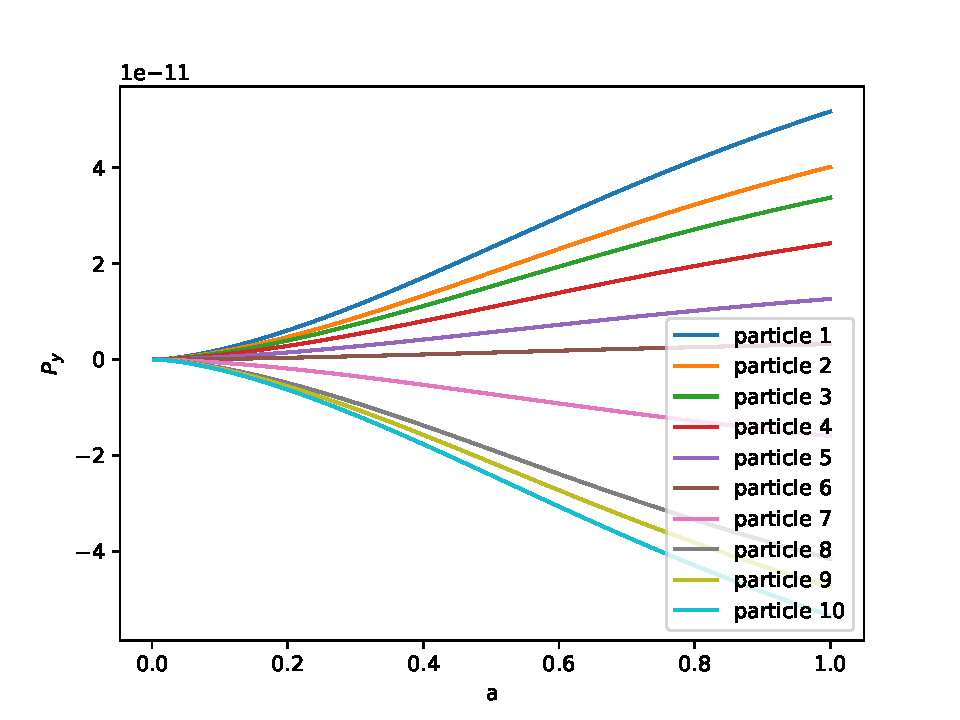
\includegraphics[width=14cm, height=8.5cm]{./Plots/4c_momentum.pdf}
\caption{The momentum of the first 10 particles as function of the scale factor. The fact that about halve of the particles have a positive momentum and that the other halve have a negative momentum is the result of the circular boundary conditions and the created field.  }
\end{figure}
\end{quote}
\end{quote}




